\documentclass[11pt,openany]{article}

\input{algebra-preamble}
\usepackage{caption}
%Tikzpicture
\usepackage{tikz}
\usepackage{tikz-3dplot}
\usepackage{tikz-cd}
\usetikzlibrary{
	3d, % For 3D drawing
	angles,
	arrows,
	arrows.meta,
	backgrounds,
	bending,
	calc,
	decorations.pathmorphing,
	decorations.pathreplacing,
	decorations.markings,
	fit,
	matrix,
	patterns,
	patterns.meta,
	positioning,
	quotes,
	shadows,
	shapes,
	shapes.geometric
}

\newcommand{\arrowboth}[1][]{\arrow[#1, bend left=15, myarrow]\arrow[bend left=15, myarrow, from=#1]}

\setstretch{1.25}
\begin{document}
	\pagenumbering{arabic}
	\begin{center}
		\huge\textbf{Groups}\\
		\vspace{0.5em}
		%	\Large\quad{대수학의 아름다움 서브-스터디}\\
		\vspace{0.5em}
		\normalsize{\today}\\
	\end{center}
\begin{center}
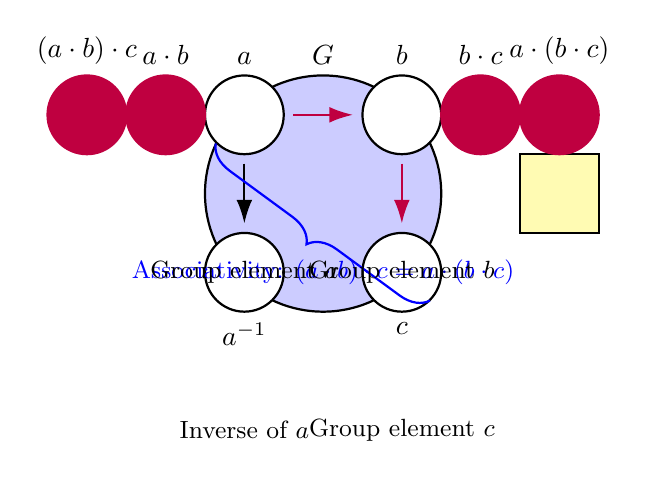
\begin{tikzpicture}[
	group/.style={draw, circle, minimum size=3cm, thick, fill=blue!20},
	element/.style={draw, circle, minimum size=1cm, thick, fill=white},
	operation/.style={font=\large, draw, rectangle, minimum size=1cm, fill=yellow!30, thick},
	arrow/.style={thick, -{Latex[length=3mm, width=2mm]}, shorten >=3pt, shorten <=3pt},
	id/.style={fill=green!30},
	inverse/.style={fill=red!30},
	assoc/.style={font=\small, blue, thick},
	closure/.style={font=\small, purple, thick}
	]
	
	% Group set
	\node[group, label=above:{$G$}] (G) at (0,0) {};
	
	% Elements
	\node[element, label=above:{$a$}] (a) at (-1, 1) {};
	\node[element, label=above:{$b$}] (b) at (1, 1) {};
	\node[element, label=below:{$c$}] (c) at (1, -1) {};
	\node[element, label=below:{$a^{-1}$}] (ainv) at (-1, -1) {};
	%	\node[element, id, label=left:{$e$}] (e) at (0, 0) {};
	
	% Operation
	\node[operation, label=above:{$\cdot$}] (op) at (3, 0) {};
	
	% Identity and Inverse
	%	\draw[arrow, id] (a) to[out=-30, in=60] node[midway, right] {} (e);
	%	\draw[arrow, id] (b) to[out=150, in=120] node[midway, left] {} (e);
	\draw[arrow, inverse] (a) -- (ainv);
	
	% Closure
	\draw[arrow, closure] (a) -- (b);
	\draw[arrow, closure] (b) -- (c);
	
	% Associativity
	\draw[assoc, decorate, decoration={brace, amplitude=10pt, mirror}] (a.south west) -- (c.south east) node[midway, below, yshift=-10pt] {Associativity: $(a \cdot b) \cdot c = a \cdot (b \cdot c)$};
	
	% Closure property illustration
	\node[element, closure, label=above:{$a \cdot b$}] (ab) at (-2, 1) {};
	\node[element, closure, label=above:{$b \cdot c$}] (bc) at (2, 1) {};
	\node[element, closure, label=above:{$(a \cdot b) \cdot c$}] (abc1) at (-3, 1) {};
	\node[element, closure, label=above:{$a \cdot (b \cdot c)$}] (abc2) at (3, 1) {};
	
	\draw[arrow, closure] (a) -- (ab);
	\draw[arrow, closure] (b) -- (bc);
	\draw[arrow, closure] (ab) -- (abc1);
	\draw[arrow, closure] (bc) -- (abc2);
	
	% Labels
	\node[below of=a, node distance=2cm, font=\small] (la) {Group element $a$};
	\node[below of=ainv, node distance=2cm, font=\small] (lainv) {Inverse of $a$};
	%	\node[below of=e, node distance=2cm, font=\small] (le) {Identity element $e$};
	\node[below of=b, node distance=2cm, font=\small] (lb) {Group element $b$};
	\node[below of=c, node distance=2cm, font=\small] (lc) {Group element $c$};
	
\end{tikzpicture}
\end{center}

\begin{center}
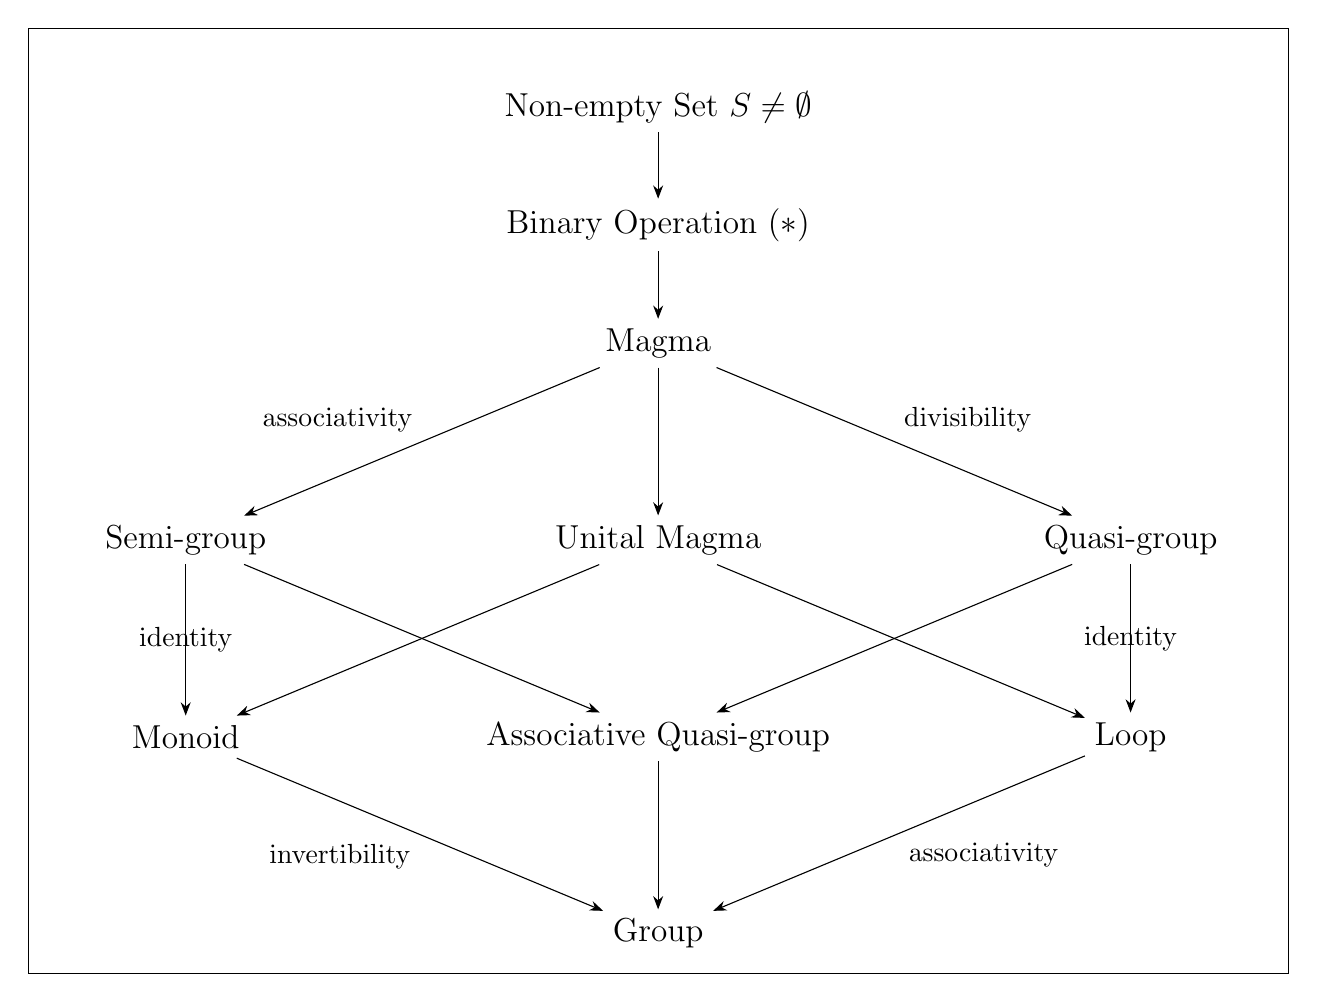
\begin{tikzpicture}[-Stealth]
	% Root node
	\draw (-8,4) rectangle (8,-8);
	\node[centered] (set) at (0,3) {\large Non-empty Set $S\neq\emptyset$};
	\node[centered] (bi-op) at (0,1.5) {\large Binary Operation ($*$)};
	\node[centered] (magma) at (0,0) {\large Magma};
	
	% First level
	\node[centered] (semi) at (-6,-2.5) {\large Semi-group};
	\node[centered] (unital) at (0,-2.5) {\large Unital Magma};
	\node[centered] (quasi) at (6,-2.5) {\large Quasi-group};
	
	% Second level 
	\node[centered] (monoid) at (-6,-5) {\large Monoid};
	\node[centered] (asso-quasi) at (0,-5) {\large Associative Quasi-group};
	\node[centered] (loop) at (6,-5) {\large Loop};
	
	% Third level of subsets
	\node[centered] (group) at (0,-7.5) {\large Group};
	
	% Level 1
	\draw (set) -- (bi-op) node[] {};
	\draw (bi-op) -- (magma) node[] {};
	\draw (magma) -- (semi) node[midway, above left] {associativity};
	\draw (magma) -- (quasi) node[midway, above right] {divisibility};
	\draw (magma) -- (unital) node[] {};
	
	% Level 2
	\draw (semi) -- (monoid) node[midway] {identity};
	\draw (semi) -- (asso-quasi) node[] {};
	\draw (quasi) -- (loop) node[midway] {identity};
	\draw (quasi) -- (asso-quasi) node[] {};
	\draw (unital) -- (monoid) node[] {};
	\draw (unital) -- (loop) node[] {};
	
	% Level 3
	\draw (monoid) -- (group) node[midway, below left] {invertibility};
	\draw (loop) -- (group) node[midway, below right] {associativity};
	\draw (asso-quasi) -- (group) node[] {};
\end{tikzpicture}
\end{center}

\newpage
\begin{table}[h!]\centering\setstretch{2.25}\adjustbox{scale=.75}{\begin{tabular}{|>{\centering\arraybackslash}m{2cm}|c|>{\centering\arraybackslash}m{3cm}||>{\centering\arraybackslash}m{3.5cm}|c|>{\centering\arraybackslash}m{3.25cm}||c|} \hline 
			Name & Group (Set) & Operation & Form of Element & Identity & Inverse & Abelian \\ \hline\hline
			Integers & $\Z$ & Addition & $k$ & $0$ & $-k$ & \vmark \\ \hline
			Integers modulo n & $\Z_n$ & Addition mod $n$ & $k$ & $0$ & $n-k$ & \vmark \\ \hline
			Rational Numbers & $\Q$ & Multiplication & $m/n$ & $1$ & $n/m$ & \vmark \\ \hline
			Real Numbers & $\R^*$ & Multiplication & $x$ & $1$ & $1/x$ & \vmark \\ \hline
			Complex Numbers & $\C^*$ & Multiplication & $a+bi$ & $1$ & $\displaystyle\frac{1}{a^2+b^2}a-\frac{1}{a^2+b^2}bi$ & \vmark \\ \hline
			Vector Space & $\R^n$ & Componentwise addition & $(a_1,a_2,\dots,a_n)$ & $(0,0,\dots,0)$ & $(-a_1,-a_2,\dots,-a_n)$ & \vmark \\ \hline
			%		$U(n)$ & Multiplication & $k,\gcd(k,n)$ & $1$ & Solution to $kx\bmod n =1$ & $\vmark$
			General Linear Group & $GL(2,F)$ & Matrix multiplication & $\begin{bsmallmatrix}
				\displaystyle a & \displaystyle b \\ \displaystyle c & \displaystyle d
			\end{bsmallmatrix}$ with $ad-bc\neq 0$ & $\begin{bsmallmatrix}\setlength{\arraycolsep}{.5cm}
				\displaystyle1 & \displaystyle0 \\ \displaystyle0 & \displaystyle1
			\end{bsmallmatrix}$ & $\begin{bsmallmatrix}
				\displaystyle\frac{d}{ad-bc} & \displaystyle \frac{-b}{ad-bc} \\
				\displaystyle\frac{-c}{ad-bc} & \displaystyle \frac{a}{ad-bc}
			\end{bsmallmatrix}$ & \xmark \\ \hline
			Special Linear Group & $SL(2,F)$ & Matrix multiplication & $\begin{bsmallmatrix}
				\displaystyle a & \displaystyle b \\ \displaystyle c & \displaystyle d
			\end{bsmallmatrix}$ with $ad-bc = 1$ & $\begin{bsmallmatrix}\setlength{\arraycolsep}{.5cm}
				\displaystyle1 & \displaystyle0 \\ \displaystyle0 & \displaystyle1
			\end{bsmallmatrix}$ & $\begin{bsmallmatrix}
				\displaystyle d & \displaystyle -b \\
				\displaystyle -c & \displaystyle a
			\end{bsmallmatrix}$ & \xmark \\ \hline
			Symmetric Group & $S_n$ & Composition of permutations & Permutations of $n$ element: $\sigma\in S_n$ & Identity permutation $e$ & Inverse permutation $\sigma^{-1}$ & \xmark \\ \hline
			Dihedral Group & $D_n$ & Composition of symmetries & Rotations $r^k$ and reflections $sr^k$, $k\in\set{0,1,\dots,n-1}$ & Identity symmetry $e$ & $r^{-k}=r^{n-k}$, $(sr^k)^{-1}=sr^{-k}$ & \xmark \\ \hline
			Quaternion Group & $Q_8$ & Quaternion multiplication & Quaternions: \( \pm 1, \pm i, \pm j, \pm k \) & $1$ & \(-a\) for \( a \in \{i, j, k\} \), \( -1 = 1^{-1}, -i = i^{-1}, -j = j^{-1}, -k = k^{-1} \) & \xmark \\ \hline
	\end{tabular}}
\end{table}

\newpage

\section*{Symmetric Groups}
\begin{table}[h!]\centering\setstretch{1.25}\begin{tabular}{c||c|c|c|c|c|c} \hline
	& $e$ & $(12)$ & $(23)$ & $(13)$ & $(123)$ & $(132)$ \\ \hline\hline
	$e$ & $e$ & $(12)$ & $(23)$ & $(13)$ & $(123)$ & $(132)$ \\ \hline
	$(12)$ & $(12)$ & $e$ & $(123)$ & $(132)$ & $(23)$ & $(13)$ \\ \hline
	$(23)$ & $(23)$ & $(132)$ & $e$ & $(123)$ & $(13)$ & $(12)$ \\ \hline
	$(13)$ & $(13)$ & $(123)$ & $(132)$ & $e$ & $(12)$ & $(23)$ \\ \hline
	$(123)$ & $(123)$ & $(13)$ & $(12)$ & $(23)$ & $(132)$ & $e$ \\ \hline
	$(132)$ & $(132)$ & $(23)$ & $(13)$ & $(12)$ & $e$ & $(123)$ \\ \hline
	\end{tabular}
\caption{Symmetric Group $S_3$}
\end{table}
\begin{center}
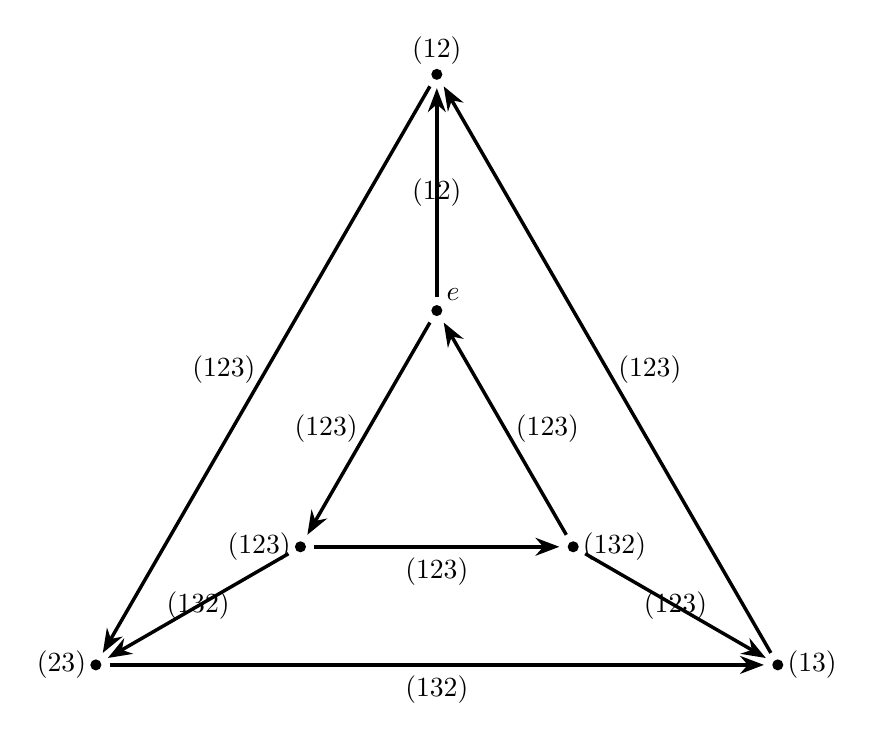
\begin{tikzpicture}
	
	% Define the radii of the circles
	\def\rA{2}
	\def\rB{5}
	
	% Draw circles
%	\draw[] (0,0) circle (\rA);
%	\draw[] (0,0) circle (\rB);
	
	% Outer triangle vertices
	\coordinate (A) at (90:\rB);
	\coordinate (B) at (210:\rB);
	\coordinate (C) at (330:\rB);
	
	% Inner triangle vertices
	\coordinate (D) at (90:\rA);
	\coordinate (E) at (210:\rA);
	\coordinate (F) at (330:\rA);
	
	% Draw nodes and labels
	\node[above] at (A) {$(12)$};
	\node[left] at (B) {$(23)$};
	\node[right] at (C) {$(13)$};
	\node[above right] at (D) {$e$};
	\node[left] at (E) {$(123)$};
	\node[right] at (F) {$(132)$};
	
	% Define a bigger arrow tip
	\tikzset{big arrow/.style={-Stealth, line width=1.25pt, scale=1, shorten <= 5pt, shorten >= 5pt}}
	
	% Draw outer triangle with bigger arrows
	\draw[big arrow] (A) -- (B) node[midway, left] {$(123)$};
	\draw[big arrow] (B) -- (C) node[midway, below] {$(132)$};
	\draw[big arrow] (C) -- (A) node[midway, right] {$(123)$};
	
	% Draw inner triangle with bigger arrows
	\draw[big arrow] (D) -- (E) node[midway, left] {$(123)$};
	\draw[big arrow] (E) -- (F) node[midway, below] {$(123)$};
	\draw[big arrow] (F) -- (D) node[midway, right] {$(123)$};
	
	\draw[big arrow] (D) -- (A) node[midway] {$(12)$};
	\draw[big arrow] (E) -- (B) node[midway] {$(132)$};
	\draw[big arrow] (F) -- (C) node[midway] {$(123)$};
	
	% Draw nodes for clarity
	\foreach \point in {A, B, C, D, E, F}
	\fill [black] (\point) circle (2pt);
	
	
\end{tikzpicture}
\end{center}
\newpage
\adjustbox{scale=.7}{
\begin{tabular}{|>{\centering\arraybackslash}m{4cm}|>{\centering\arraybackslash}m{3cm}|>{\centering\arraybackslash}m{3cm}|>{\centering\arraybackslash}m{1.5cm}|>{\centering\arraybackslash}m{1.5cm}|>{\centering\arraybackslash}m{2cm}|>{\centering\arraybackslash}m{2cm}|}
	\hline
	\textbf{Ring (Set)} & \textbf{Addition Operation} & \textbf{Multiplication Operation} & \textbf{Additive Identity} & \textbf{Multiplicative Identity} & \textbf{Form of Element} & \textbf{Commutative} \\
	\hline
	Integers \( \mathbb{Z} \) & Standard addition \( + \) & Standard multiplication \( \cdot \) & \( 0 \) & \( 1 \) & Integers & Yes \\
	\hline
	Real Numbers \( \mathbb{R} \) & Standard addition \( + \) & Standard multiplication \( \cdot \) & \( 0 \) & \( 1 \) & Real numbers & Yes \\
	\hline
	Complex Numbers \( \mathbb{C} \) & Standard addition \( + \) & Standard multiplication \( \cdot \) & \( 0 \) & \( 1 \) & \( a + bi \) where \( a, b \in \mathbb{R} \) & Yes \\
	\hline
	Polynomials with Real Coefficients \( \mathbb{R}[x] \) & Polynomial addition & Polynomial multiplication & \( 0 \) (zero polynomial) & \( 1 \) (constant polynomial) & \( a_n x^n + \cdots + a_1 x + a_0 \) & Yes \\
	\hline
	Matrices \( M_n(\mathbb{R}) \) & Matrix addition & Matrix multiplication & Zero matrix & Identity matrix & \( n \times n \) matrices & No \\
	\hline
	Integers Modulo \( n \) \( \mathbb{Z}/n\mathbb{Z} \) & Addition modulo \( n \) & Multiplication modulo \( n \) & \( 0 \) & \( 1 \) & \( \{ 0, 1, \ldots, n-1 \} \) & Yes \\
	\hline
\end{tabular}}
\begin{center}
\begin{tabular}{|>{\centering\arraybackslash}m{3cm}|>{\centering\arraybackslash}m{2cm}|>{\centering\arraybackslash}m{1.5cm}|>{\centering\arraybackslash}m{4cm}|>{\centering\arraybackslash}m{4cm}|>{\centering\arraybackslash}m{1.5cm}|}
	\hline
	\textbf{Group (Set)} & \textbf{Operation} & \textbf{Identity} & \textbf{Form of Element} & \textbf{Normal Subgroups} & \textbf{Abelian} \\
	\hline
	Symmetric Group \( S_3 \) & Composition of permutations & Identity permutation \( e \) & Permutations of 3 elements & \(\{ e, (123), (132) \}\), \(\{ e, (12), (13), (23), (123), (132) \}\) & No \\
	\hline
	Dihedral Group \( D_4 \) & Composition of symmetries & Identity symmetry \( e \) & Rotations \( r^k \) and reflections \( sr^k \), \( k \in \{0, 1, 2, 3\} \) & \(\{ e, r, r^2, r^3 \}\), \(\{ e, r^2, s, sr^2 \}\) & No \\
	\hline
	Quaternion Group \( Q_8 \) & Quaternion multiplication & \( 1 \) & Quaternions \( \pm 1, \pm i, \pm j, \pm k \) & \(\{ 1, -1 \}\), \(\{ 1, -1, i, -i \}\), \(\{ 1, -1, j, -j \}\), \(\{ 1, -1, k, -k \}\) & No \\
	\hline
	Integers Modulo \( n \) \( \mathbb{Z}/n\mathbb{Z} \) & Addition modulo \( n \) & \( 0 \) & \( \{0, 1, \ldots, n-1\} \) & All subgroups are normal & Yes \\
	\hline
\end{tabular}
\end{center}
\adjustbox{scale=.5}{
\begin{tabular}{ccccccc}
	\hline
	\textbf{Ring (Set)} & \textbf{Addition Operation} & \textbf{Multiplication Operation} & \textbf{Additive Identity} & \textbf{Multiplicative Identity} & \textbf{Form of Element} \\
	\hline
	Matrices \( M_n(\mathbb{R}) \) & Matrix addition & Matrix multiplication & Zero matrix & Identity matrix & \( n \times n \) matrices \\
	\hline
	Quaternions \( \mathbb{H} \) & Quaternion addition & Quaternion multiplication & \( 0 \) & \( 1 \) & \( a + bi + cj + dk \) where \( a, b, c, d \in \mathbb{R} \) \\
	\hline
	Differential Operators & Operator addition & Operator composition & Zero operator & Identity operator & \( \sum a_i \frac{d^i}{dx^i} \) \\
	\hline
	Group Rings \( \mathbb{R}[G] \) & Group ring addition & Group ring multiplication & Zero element & Identity element & \( \sum a_g g \) where \( a_g \in \mathbb{R} \) and \( g \in G \) \\
	\hline
	Endomorphism Rings \( \text{End}(V) \) & Function addition & Function composition & Zero map & Identity map & Linear transformations on vector space \( V \) \\
	\hline
	Octonions \( \mathbb{O} \) & Octonion addition & Octonion multiplication & \( 0 \) & \( 1 \) & \( a + b e_1 + c e_2 + d e_3 + e e_4 + f e_5 + g e_6 + h e_7 \) where \( a, b, c, d, e, f, g, h \in \mathbb{R} \) \\
	\hline
\end{tabular}}
\begin{center}
\begin{tabular}{|>{\centering\arraybackslash}m{4cm}|>{\centering\arraybackslash}m{2cm}|>{\centering\arraybackslash}m{2cm}|>{\centering\arraybackslash}m{2cm}|>{\centering\arraybackslash}m{2cm}|}
	\hline
	\textbf{Type} & \textbf{Ideal} & \textbf{Principal Ideal} & \textbf{Prime Ideal} & \textbf{Maximal Ideal} \\
	\hline
	\textbf{Definition} & A subset closed under addition and multiplication by any ring element & An ideal generated by a single element & An ideal where if \(ab \in I\), then \(a \in I\) or \(b \in I\) & An ideal such that there are no larger ideals except the ring itself \\
	\hline
	Is an Ideal & \(O\) & \(O\) & \(O\) & \(O\) \\
	\hline
	Can be Principal & \(O\) & \(O\) & \(O\) & \(O\) \\
	\hline
	Is Prime & \(X\) & \(X\) & \(O\) & \(O\) \\
	\hline
	Is Maximal & \(X\) & \(X\) & \(X\) & \(O\) \\
	\hline
\end{tabular}
\end{center}

\begin{center}
\begin{tabular}{|>{\centering\arraybackslash}m{4cm}|>{\centering\arraybackslash}m{3cm}|>{\centering\arraybackslash}m{3cm}|>{\centering\arraybackslash}m{3cm}|}
	\hline
	\textbf{Ring (Set)} & \textbf{Principal Ideals} & \textbf{Prime Ideals} & \textbf{Maximal Ideals} \\
	\hline
	\(\mathbb{Z}\) & \((2), (3), (5)\) & \((2), (3), (5)\) & \((2), (3), (5)\) \\
	\hline
	\(\mathbb{R}[x]\) & \((x), (x-1), (x^2+1)\) & \((x)\) & \((x-1)\) \\
	\hline
	\(\mathbb{C}[x]\) & \((x), (x-i), (x+i)\) & \((x-i), (x+i)\) & \((x-i), (x+i)\) \\
	\hline
	\(\mathbb{Z}/6\mathbb{Z}\) & \((2), (3)\) & None & \((2), (3)\) \\
	\hline
	\(\mathbb{Z}[i]\) & \((1+i), (2)\) & \((1+i)\) & \((1+i)\) \\
	\hline
	\(\mathbb{Z}/p\mathbb{Z}\) where \(p\) is prime & \((0), (1)\) & \((0)\) & \((0)\) \\
	\hline
	\(\mathbb{R}\) & \((0)\) & None & \((0)\) \\
	\hline
	\(\mathbb{C}\) & \((0)\) & None & \((0)\) \\
	\hline
	\(\mathbb{Z}[x]\) & \((2), (3), (x)\) & \((x), (2)\) & None \\
	\hline
	\(M_n(\mathbb{R})\) & \((E_{11})\) & None & None \\
	\hline
	\(\mathbb{H}\) (Quaternions) & \((1+i)\) & None & None \\
	\hline
\end{tabular}
\end{center}

\begin{center}
\begin{tabular}{|>{\centering\arraybackslash}m{4cm}|>{\centering\arraybackslash}m{4cm}|>{\centering\arraybackslash}m{4cm}|>{\centering\arraybackslash}m{4cm}|}
	\hline
	\textbf{Ring (Set)} & \textbf{Principal Ideals} & \textbf{Prime Ideals} & \textbf{Maximal Ideals} \\
	\hline
	\(\mathbb{Z}\) & \((2) = \{2k \mid k \in \mathbb{Z}\}\) & \((2) = \{2k \mid k \in \mathbb{Z}\}\) & \((2) = \{2k \mid k \in \mathbb{Z}\}\) \\
	& \((3) = \{3k \mid k \in \mathbb{Z}\}\) & \((3) = \{3k \mid k \in \mathbb{Z}\}\) & \((3) = \{3k \mid k \in \mathbb{Z}\}\) \\
	& \((5) = \{5k \mid k \in \mathbb{Z}\}\) & \((5) = \{5k \mid k \in \mathbb{Z}\}\) & \((5) = \{5k \mid k \in \mathbb{Z}\}\) \\
	\hline
	\(\mathbb{R}[x]\) & \((x) = \{x f(x) \mid f(x) \in \mathbb{R}[x]\}\) & \((x) = \{x f(x) \mid f(x) \in \mathbb{R}[x]\}\) & \((x-1) = \{(x-1) f(x) \mid f(x) \in \mathbb{R}[x]\}\) \\
	& \((x-1) = \{(x-1) f(x) \mid f(x) \in \mathbb{R}[x]\}\) &  &  \\
	& \((x^2+1) = \{(x^2+1) f(x) \mid f(x) \in \mathbb{R}[x]\}\) &  &  \\
	\hline
	\(\mathbb{C}[x]\) & \((x) = \{x f(x) \mid f(x) \in \mathbb{C}[x]\}\) & \((x-i) = \{(x-i) f(x) \mid f(x) \in \mathbb{C}[x]\}\) & \((x-i) = \{(x-i) f(x) \mid f(x) \in \mathbb{C}[x]\}\) \\
	& \((x-i) = \{(x-i) f(x) \mid f(x) \in \mathbb{C}[x]\}\) & \((x+i) = \{(x+i) f(x) \mid f(x) \in \mathbb{C}[x]\}\) & \((x+i) = \{(x+i) f(x) \mid f(x) \in \mathbb{C}[x]\}\) \\
	& \((x+i) = \{(x+i) f(x) \mid f(x) \in \mathbb{C}[x]\}\) &  &  \\
	\hline
	\(\mathbb{Z}/6\mathbb{Z}\) & \((2) = \{0, 2, 4\}\) & None & \((2) = \{0, 2, 4\}\) \\
	& \((3) = \{0, 3\}\) &  & \((3) = \{0, 3\}\) \\
	\hline
	\(\mathbb{Z}[i]\) & \((1+i) = \{(1+i) z \mid z \in \mathbb{Z}[i]\}\) & \((1+i) = \{(1+i) z \mid z \in \mathbb{Z}[i]\}\) & \((1+i) = \{(1+i) z \mid z \in \mathbb{Z}[i]\}\) \\
	& \((2) = \{2 z \mid z \in \mathbb{Z}[i]\}\) &  &  \\
	\hline
	\(\mathbb{Z}/p\mathbb{Z}\) where \(p\) is prime & \((0) = \{0\}\) & \((0) = \{0\}\) & \((0) = \{0\}\) \\
	& \((1) = \mathbb{Z}/p\mathbb{Z}\) &  &  \\
	\hline
	\(\mathbb{R}\) & \((0) = \{0\}\) & None & \((0) = \{0\}\) \\
	\hline
	\(\mathbb{C}\) & \((0) = \{0\}\) & None & \((0) = \{0\}\) \\
	\hline
	\(\mathbb{Z}[x]\) & \((2) = \{2 f(x) \mid f(x) \in \mathbb{Z}[x]\}\) & \((2) = \{2 f(x) \mid f(x) \in \mathbb{Z}[x]\}\) & None \\
	& \((3) = \{3 f(x) \mid f(x) \in \mathbb{Z}[x]\}\) &  &  \\
	& \((x) = \{x f(x) \mid f(x) \in \mathbb{Z}[x]\}\) & \((x) = \{x f(x) \mid f(x) \in \mathbb{Z}[x]\}\) &  \\
	\hline
	\(M_n(\mathbb{R})\) & \((E_{11}) = \{A E_{11} B \mid A, B \in M_n(\mathbb{R})\}\) & None & None \\
	\hline
	\(\mathbb{H}\) (Quaternions) & \((1+i) = \{(1+i) q \mid q \in \mathbb{H}\}\) & None & None \\
	\hline
\end{tabular}
\end{center}

\begin{center}
\begin{tabular}{|>{\centering\arraybackslash}m{4cm}|>{\centering\arraybackslash}m{4cm}|>{\centering\arraybackslash}m{4cm}|>{\centering\arraybackslash}m{4cm}|}
	\hline
	\textbf{Ring (Set)} & \textbf{Principal Ideals} & \textbf{Prime Ideals} & \textbf{Maximal Ideals} \\
	\hline
	\(\mathbb{Z}\) & \((2) = \{2k \mid k \in \mathbb{Z}\}\) & \((2) = \{2k \mid k \in \mathbb{Z}\}\) & \((2) = \{2k \mid k \in \mathbb{Z}\}\) \\
	& \((3) = \{3k \mid k \in \mathbb{Z}\}\) & \((3) = \{3k \mid k \in \mathbb{Z}\}\) & \((3) = \{3k \mid k \in \mathbb{Z}\}\) \\
	& \((5) = \{5k \mid k \in \mathbb{Z}\}\) & \((5) = \{5k \mid k \in \mathbb{Z}\}\) & \((5) = \{5k \mid k \in \mathbb{Z}\}\) \\
	\hline
	\(\mathbb{R}[x]\) & \((x) = \{x f(x) \mid f(x) \in \mathbb{R}[x]\}\) & \((x)\) & \((x-1)\) \\
	& \((x-1) = \{(x-1) f(x) \mid f(x) \in \mathbb{R}[x]\}\) &  &  \\
	& \((x^2+1) = \{(x^2+1) f(x) \mid f(x) \in \mathbb{R}[x]\}\) &  &  \\
	\hline
	\(\mathbb{C}[x]\) & \((x) = \{x f(x) \mid f(x) \in \mathbb{C}[x]\}\) & \((x-i)\) & \((x-i)\) \\
	& \((x-i) = \{(x-i) f(x) \mid f(x) \in \mathbb{C}[x]\}\) & \((x+i)\) & \((x+i)\) \\
	& \((x+i) = \{(x+i) f(x) \mid f(x) \in \mathbb{C}[x]\}\) &  &  \\
	\hline
	\(\mathbb{Z}/6\mathbb{Z}\) & \((2) = \{0, 2, 4\}\) & None & \((2) = \{0, 2, 4\}\) \\
	& \((3) = \{0, 3\}\) &  & \((3) = \{0, 3\}\) \\
	\hline
	\(\mathbb{Z}[i]\) & \((1+i) = \{(1+i) z \mid z \in \mathbb{Z}[i]\}\) & \((1+i)\) & \((1+i)\) \\
	& \((2) = \{2 z \mid z \in \mathbb{Z}[i]\}\) &  &  \\
	\hline
	\(\mathbb{Z}/p\mathbb{Z}\) where \(p\) is prime & \((0) = \{0\}\) & \((0)\) & \((0)\) \\
	& \((1) = \mathbb{Z}/p\mathbb{Z}\) &  &  \\
	\hline
	\(\mathbb{R}\) & \((0) = \{0\}\) & None & \((0)\) \\
	\hline
	\(\mathbb{C}\) & \((0) = \{0\}\) & None & \((0)\) \\
	\hline
	\(\mathbb{Z}[x]\) & \((2) = \{2 f(x) \mid f(x) \in \mathbb{Z}[x]\}\) & \((2)\) & None \\
	& \((3) = \{3 f(x) \mid f(x) \in \mathbb{Z}[x]\}\) &  &  \\
	& \((x) = \{x f(x) \mid f(x) \in \mathbb{Z}[x]\}\) & \((x)\) &  \\
	\hline
	\(M_n(\mathbb{R})\) & \((E_{11}) = \{A E_{11} B \mid A, B \in M_n(\mathbb{R})\}\) & None & None \\
	\hline
	\(\mathbb{H}\) (Quaternions) & \((1+i) = \{(1+i) q \mid q \in \mathbb{H}\}\) & None & None \\
	\hline
\end{tabular}
\end{center}

\newpage
\adjustbox{scale=.7}{
\begin{tabular}{|ccccc|}
	\hline
	\textbf{Ring (Set)} & \textbf{Examples of Ideals} & \textbf{Examples of Principal Ideals} & \textbf{Examples of Prime Ideals} & \textbf{Examples of Maximal Ideals} \\
	\hline
	\(\mathbb{Z}\) & \((0), (2), (3)\) & \((2) = \{2k \mid k \in \mathbb{Z}\}\) & \((2) = \{2k \mid k \in \mathbb{Z}\}\) & \((2) = \{2k \mid k \in \mathbb{Z}\}\) \\
	& \((4), (6)\) & \((3) = \{3k \mid k \in \mathbb{Z}\}\) & \((3) = \{3k \mid k \in \mathbb{Z}\}\) & \((3) = \{3k \mid k \in \mathbb{Z}\}\) \\
	& \((0)\) & \((5) = \{5k \mid k \in \mathbb{Z}\}\) & \((5) = \{5k \mid k \in \mathbb{Z}\}\) & \((5) = \{5k \mid k \in \mathbb{Z}\}\) \\
	\hline
	\(\mathbb{R}[x]\) & \((0), (x), (x-1)\) & \((x) = \{x f(x) \mid f(x) \in \mathbb{R}[x]\}\) & \((x)\) & \((x-1)\) \\
	& \((x^2+1)\) & \((x-1) = \{(x-1) f(x) \mid f(x) \in \mathbb{R}[x]\}\) &  &  \\
	&  & \((x^2+1) = \{(x^2+1) f(x) \mid f(x) \in \mathbb{R}[x]\}\) &  &  \\
	\hline
	\(\mathbb{C}[x]\) & \((0), (x), (x-i)\) & \((x) = \{x f(x) \mid f(x) \in \mathbb{C}[x]\}\) & \((x-i)\) & \((x-i)\) \\
	& \((x+i)\) & \((x-i) = \{(x-i) f(x) \mid f(x) \in \mathbb{C}[x]\}\) & \((x+i)\) & \((x+i)\) \\
	&  & \((x+i) = \{(x+i) f(x) \mid f(x) \in \mathbb{C}[x]\}\) &  &  \\
	\hline
	\(\mathbb{Z}/6\mathbb{Z}\) & \((0), (2), (3)\) & \((2) = \{0, 2, 4\}\) & None & \((2) = \{0, 2, 4\}\) \\
	&  & \((3) = \{0, 3\}\) &  & \((3) = \{0, 3\}\) \\
	\hline
	\(\mathbb{Z}[i]\) & \((0), (1+i), (2)\) & \((1+i) = \{(1+i) z \mid z \in \mathbb{Z}[i]\}\) & \((1+i)\) & \((1+i)\) \\
	&  & \((2) = \{2 z \mid z \in \mathbb{Z}[i]\}\) &  &  \\
	\hline
	\(\mathbb{Z}/p\mathbb{Z}\) where \(p\) is prime & \((0), (1)\) & \((0) = \{0\}\) & \((0)\) & \((0)\) \\
	&  & \((1) = \mathbb{Z}/p\mathbb{Z}\) &  &  \\
	\hline
	\(\mathbb{R}\) & \((0)\) & \((0) = \{0\}\) & None & \((0)\) \\
	\hline
	\(\mathbb{C}\) & \((0)\) & \((0) = \{0\}\) & None & \((0)\) \\
	\hline
	\(\mathbb{Z}[x]\) & \((0), (2), (3)\) & \((2) = \{2 f(x) \mid f(x) \in \mathbb{Z}[x]\}\) & \((2)\) & None \\
	&  & \((3) = \{3 f(x) \mid f(x) \in \mathbb{Z}[x]\}\) &  &  \\
	&  & \((x) = \{x f(x) \mid f(x) \in \mathbb{Z}[x]\}\) & \((x)\) &  \\
	\hline
	\(M_n(\mathbb{R})\) & \((0), (E_{11})\) & \((E_{11}) = \{A E_{11} B \mid A, B \in M_n(\mathbb{R})\}\) & None & None \\
	\hline
	\(\mathbb{H}\) (Quaternions) & \((0), (1+i)\) & \((1+i) = \{(1+i) q \mid q \in \mathbb{H}\}\) & None & None \\
	\hline
\end{tabular}}
\end{document}
